\documentclass[usenames,dvipsnames]{beamer}
\usepackage[utf8]{inputenc}
\usepackage{verbatim}
\usetheme{umu}

%%% Bibliography
\usepackage[style=authoryear,backend=biber]{biblatex}
\addbibresource{bibliography.bib}

% Author names in publication list are consistent 
% i.e. name1 surname1, name2 surname2
% See https://tex.stackexchange.com/questions/106914/biblatex-does-not-reverse-the-first-and-last-names-of-the-second-author
\DeclareNameAlias{author}{first-last}

%%% Suppress biblatex annoying warning
\usepackage{silence}
\WarningFilter{biblatex}{Patching footnotes failed}

\usepackage{enumitem}
\usepackage{siunitx}
\usepackage{xcolor}

%%% Some useful commands
% pdf-friendly newline in links
\newcommand{\pdfnewline}{\texorpdfstring{\newline}{ }} 
% Fill the vertical space in a slide (to put text at the bottom)
\newcommand{\framefill}{\vskip0pt plus 1filll}
\setbeamertemplate{caption}{\raggedright\insertcaption\par}

%%%%%%%%%%%%%%%%%%%%%%%%%%%%%%%%%%%%%%%%%%%%%%%%%%%%%%%%%%%%%%%%%%%%%%%%%%%%%%%%%%%%%
%%%%%%%%%%%%%%%%%%%%%%%%%%%%%%% YOUR PRESENTATION BELOW %%%%%%%%%%%%%%%%%%%%%%%%%%%%%
%%%%%%%%%%%%%%%%%%%%%%%%%%%%%%%%%%%%%%%%%%%%%%%%%%%%%%%%%%%%%%%%%%%%%%%%%%%%%%%%%%%%%
\title{Evolution of galaxy dynamics over the last 10 Gyrs with MUSE/VLT}
\date[\today]{\small\today}
\author[Mercier Wilfried]{
  \textbf{Author}: \hspace{33pt} Mercier Wilfried
  \pdfnewline
  \textbf{Supervisor}: \hspace{14pt} Contini Thierry (IRAP)
  \pdfnewline
  \textbf{Co-Supervisor}: Epinat Benoit (LAM)
  }


\institute{Observatoire de Paris}

\begin{document}

\begin{frame}
\titlepage
\end{frame}

\section{Galaxy evolution}
\begin{frame}{Galaxy evolution}
	Morphology at $z> 0.5$ different from the local Universe. \\

	Kinematics more disturbed. \\
	
	Why ?

	\vfill
	\begin{itemize}[label=$\rhd$]
		\item Impact of the environment on the kinematics ? On the morphology ? How do they scale with each other ?
		\item Which physical processes are shaping galaxies ?
		\begin{itemize}[label=$\cdot$]
			\item Which is/are dominant  ?
			\item How to identify them ?
		\end{itemize}
		\item Origin of quenching ?
		\item Ancestors of local giant spirals ?
		
	\end{itemize}
\end{frame}


\section{IFS \& MUSE}
\begin{frame}{Integral Field Spectroscopy \& MUSE}

	\begin{columns}[T]
	
		\begin{column}{0.5\linewidth}
			\underline{IFS:}
			\begin{itemize}[label=$\rhd$]
				\item 3D cubes (2D spatial + 1D spectral)
				\item photometry + kinematics
			\end{itemize}					
		
			\vspace{25pt}
			\underline{MUSE:}
			\begin{itemize}[label=$\rhd$]
				\item $1 \times \SI{1}{arcmin\squared}$ FoV
				\item $\SI{0.2}{arcsec}$ spatial sampling
				\item spectral range $[\SI{4650}{\angstrom}, \SI{9300}{\angstrom}]$
				\item seeing-limited or AO observations
			\end{itemize}
		\end{column}

		\begin{column}{0.4\linewidth}
			\begin{figure}
				\vspace{-15pt}
				\centering
				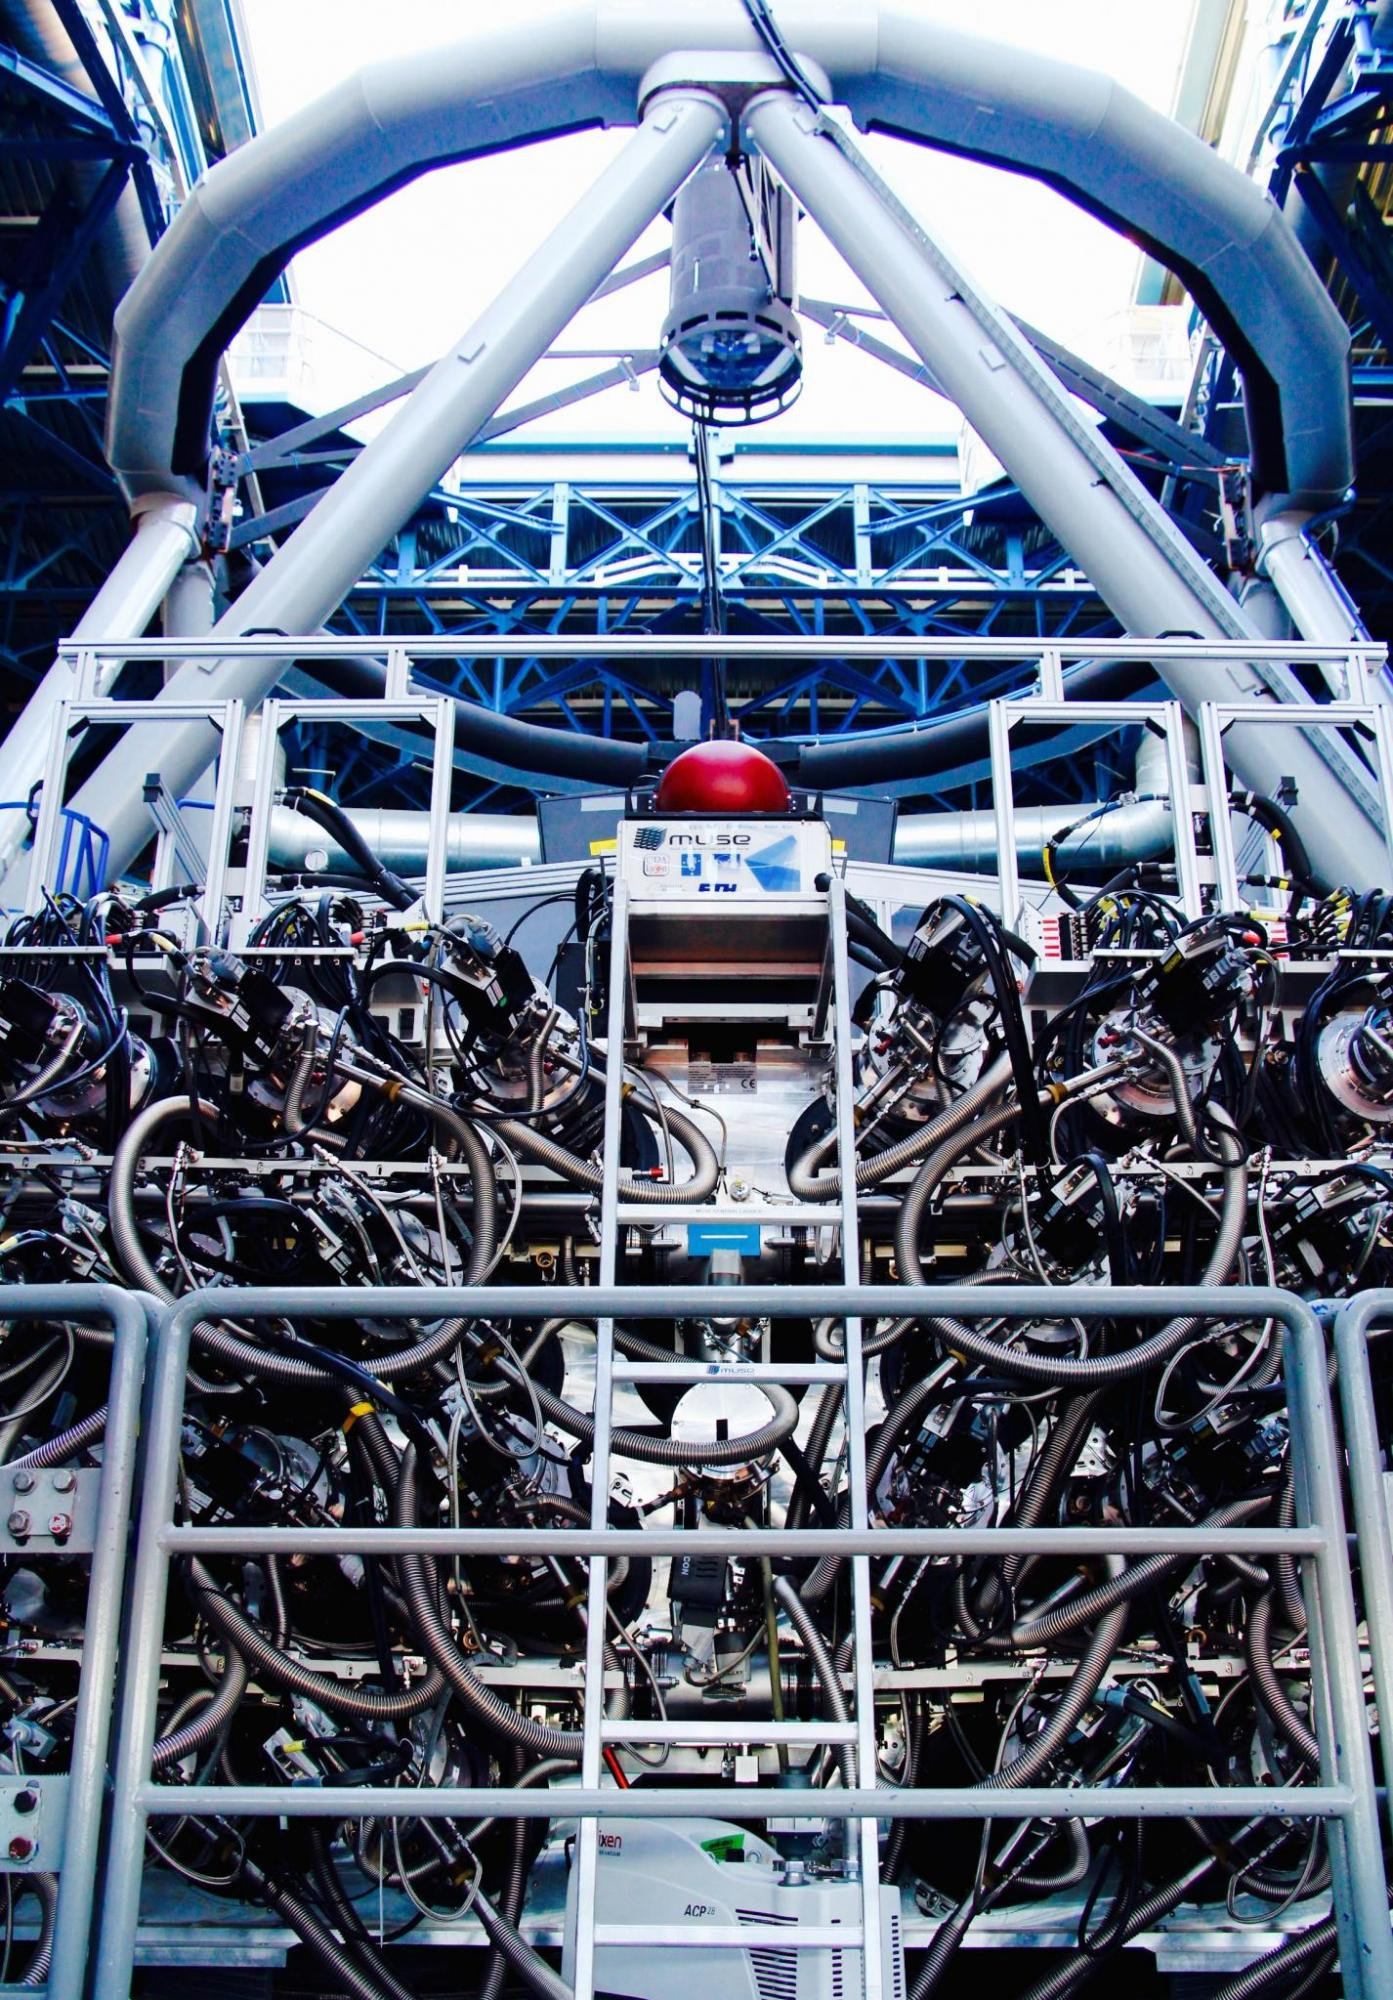
\includegraphics[width=\linewidth]{{graphics/MUSE_tcontini2}.jpg}
				\caption{MUSE instrument. Credit: Contini Thierry (IRAP)}
			\end{figure}
		\end{column}
	\end{columns}

\end{frame}


\section{Initial sample}
\begin{frame}{Our sample}
	\begin{columns}
		\begin{column}{0.5\linewidth}	
			\begin{figure}
				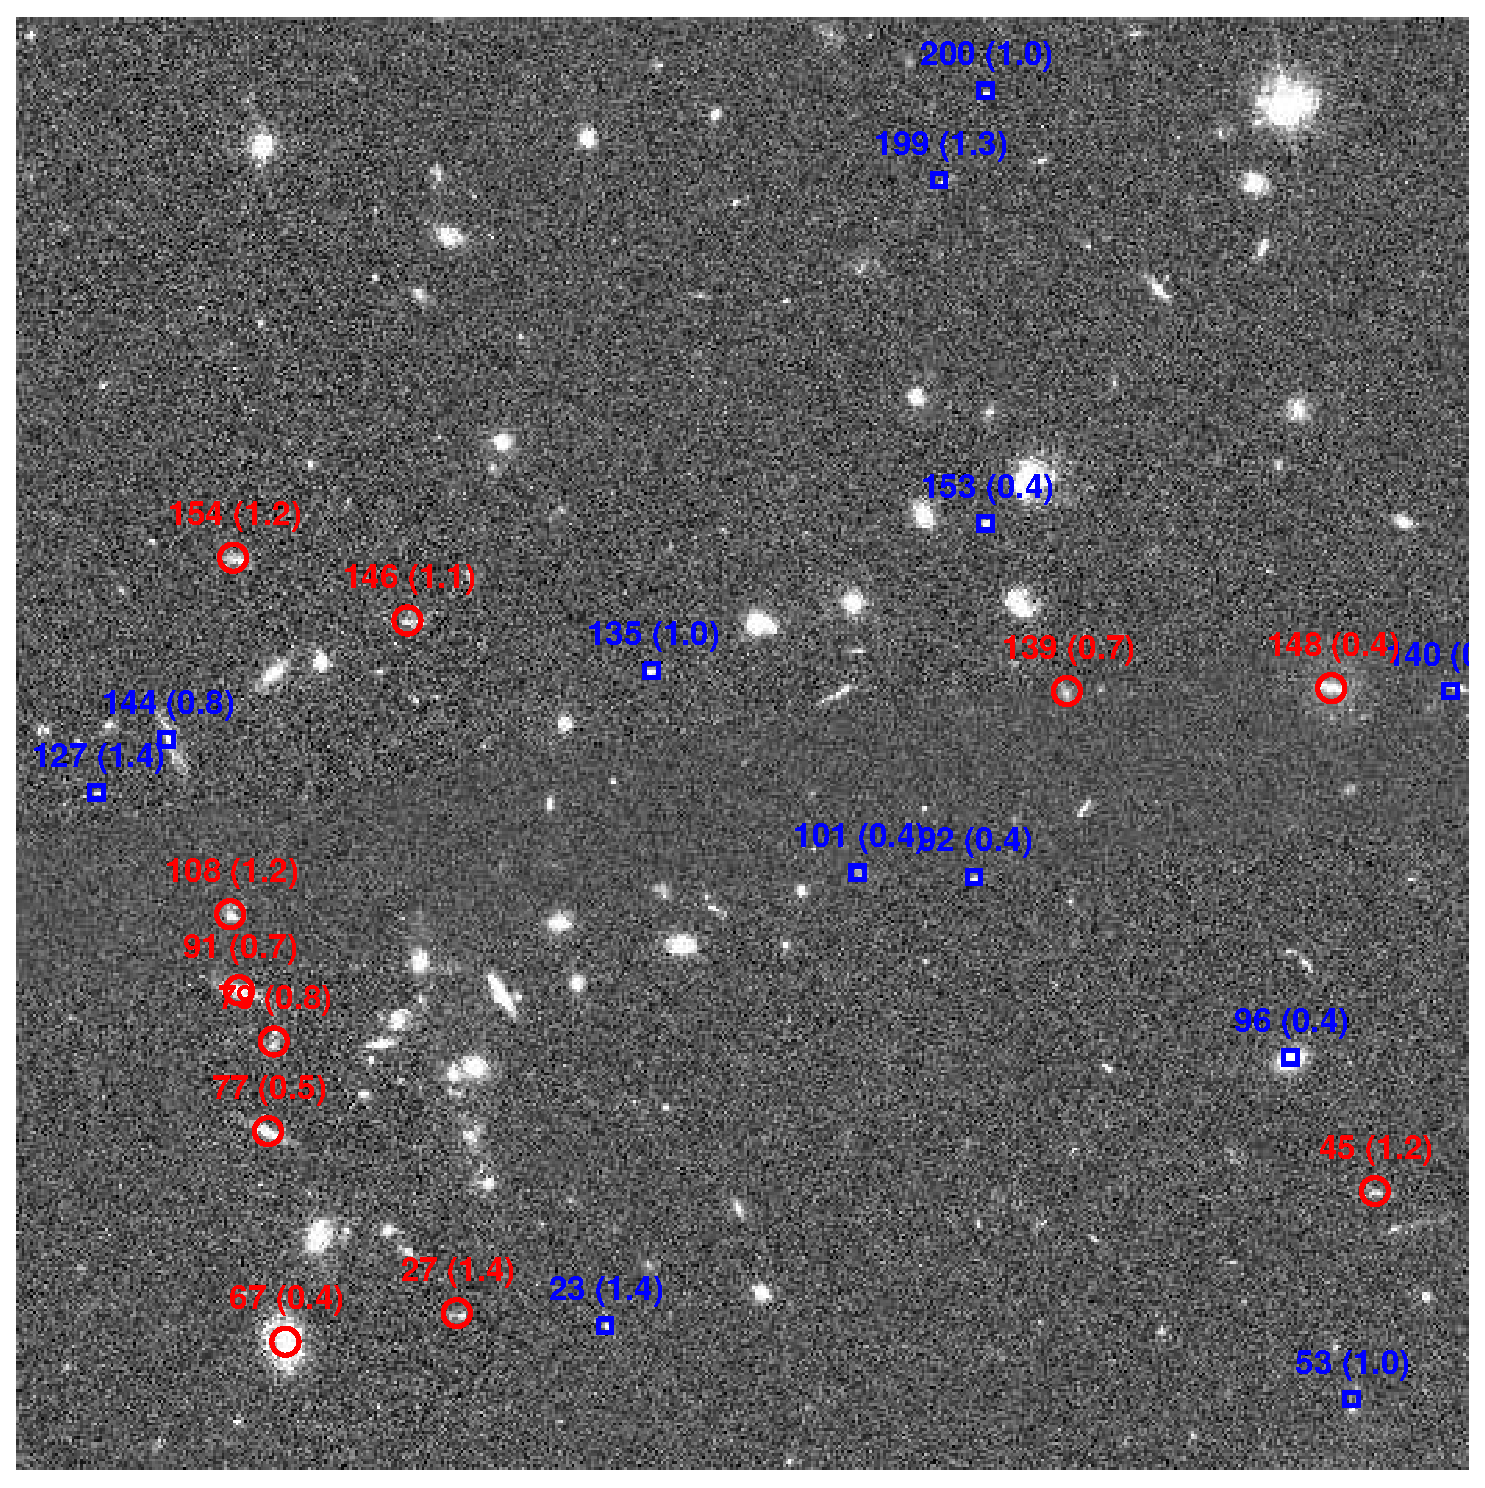
\includegraphics[width=\linewidth]{{graphics/CGr30}.eps}
				\caption{HST image of COSMOS group CGr30}
			\end{figure}
		\end{column}
		
		\hspace{-10pt}
		\begin{column}{0.5\linewidth}
			\begin{itemize}[label=$\rhd$]
				\item $16$ MUSE fields in COSMOS area
				\item exposures from $1$ to $\SI{10}{hr}$
				\item seeing-limited ($\rm{FWHM} \lesssim \SI{0.7}{"}$) or AO ($\rm{FWHM} \lesssim \SI{0.5}{"}$)
				\begin{itemize}[label=$\cdot$]
					\item \textit{deep} and \textit{best\_seeing} observations
				\end{itemize}
				\item $\sim 500$ field galaxies with [OII] detection
				\begin{itemize}[label=$\cdot$]
					\item HST-ACS counterparts
					\item $0.4 \leq z \leq 1.4$
				\end{itemize}
			\end{itemize}
		\end{column}
	\end{columns}
\end{frame}


\section{Checking morphological parameters}
\subsection{A need for reliable morphological parameters}
\begin{frame}{Checking a couple of parameters}
	\framesubtitle{A need for reliable morphological parameters}

	Morphological parameters are useful for
	
	\begin{itemize}[label=$\rhd$]
		\item the morpho-kinematics comparison
		\item \textbf{the kinematical model}
	\end{itemize}

	\vfill
	
	The two most important are
	
	\begin{itemize}[label=$\rhd$]
		\item a size measure to select resolved galaxies
		\begin{itemize}[label=$\cdot$]
			\item half-light radius $R_{1/2}$
		\end{itemize}
		\item the ellipticity
		\begin{itemize}[label=$\cdot$]
			\item compute the inclination from $\cos i = 1 - e$
			\item used as a fixed input for the kinematical model
		\end{itemize}
		
	\end{itemize}

\end{frame}

\subsection{Half-light Radius}
\begin{frame}{Checking a couple of parameters}
	\framesubtitle{Half-light radius}
	
	\begin{columns}
		\hspace{-20pt}
		\begin{column}{0.9\linewidth}
			\begin{figure}
				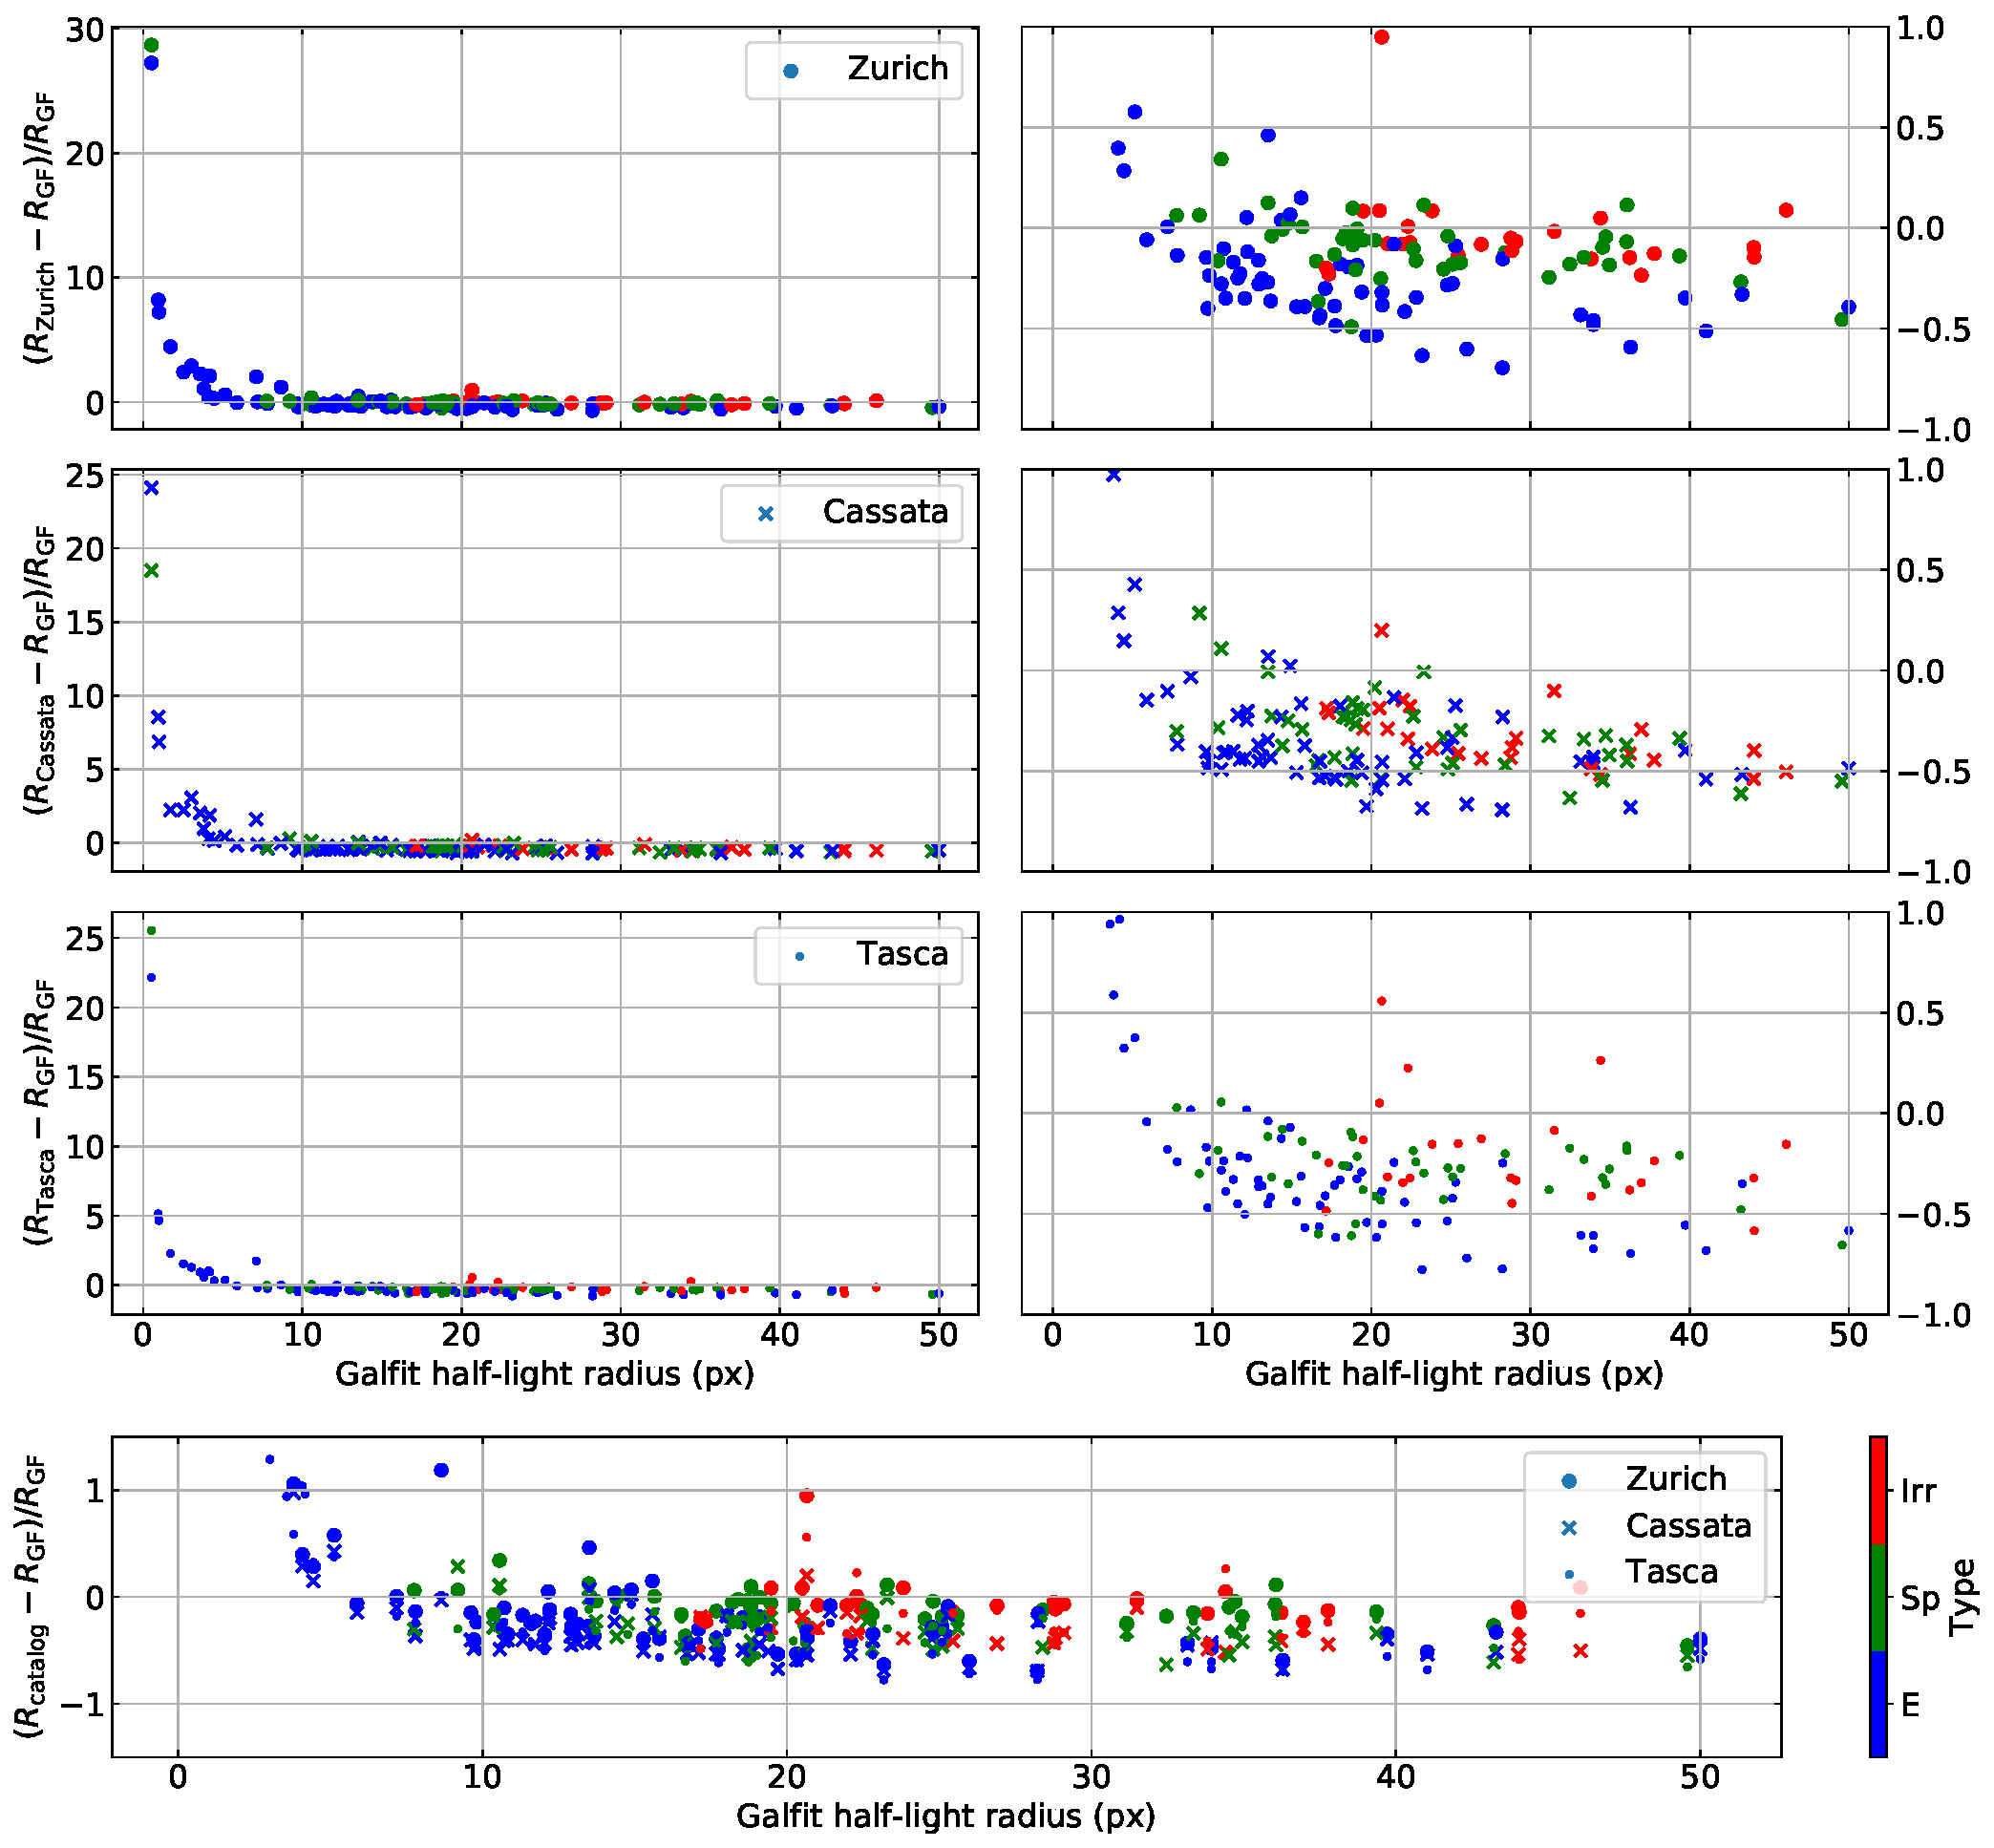
\includegraphics[width=0.85\linewidth]{{graphics/relErr_against_GalFit1.5LightRadius_colourCoded_CassataType}.pdf}
				\caption{spheroidal  \textcolor{OliveGreen}{disk-like}    \textcolor{magenta}{irregulars}}
			\end{figure}
		\end{column}
	
		\hspace{-20pt}
		\begin{column}{0.38\linewidth}	
			GALFIT run by V. Abril-Melgajero (LAM) on structure galaxies
			\begin{itemize}[label=$\rhd$]
				\item GALFIT radius used as a reference
			\end{itemize}
		\end{column}
	\end{columns}
\end{frame}




\subsection{Ellipticity}
\begin{frame}{Checking a few parameters}
	\framesubtitle{Ellipticity}
	\begin{columns}	
		\begin{column}{0.5\linewidth}
			\vspace{-10pt}		
			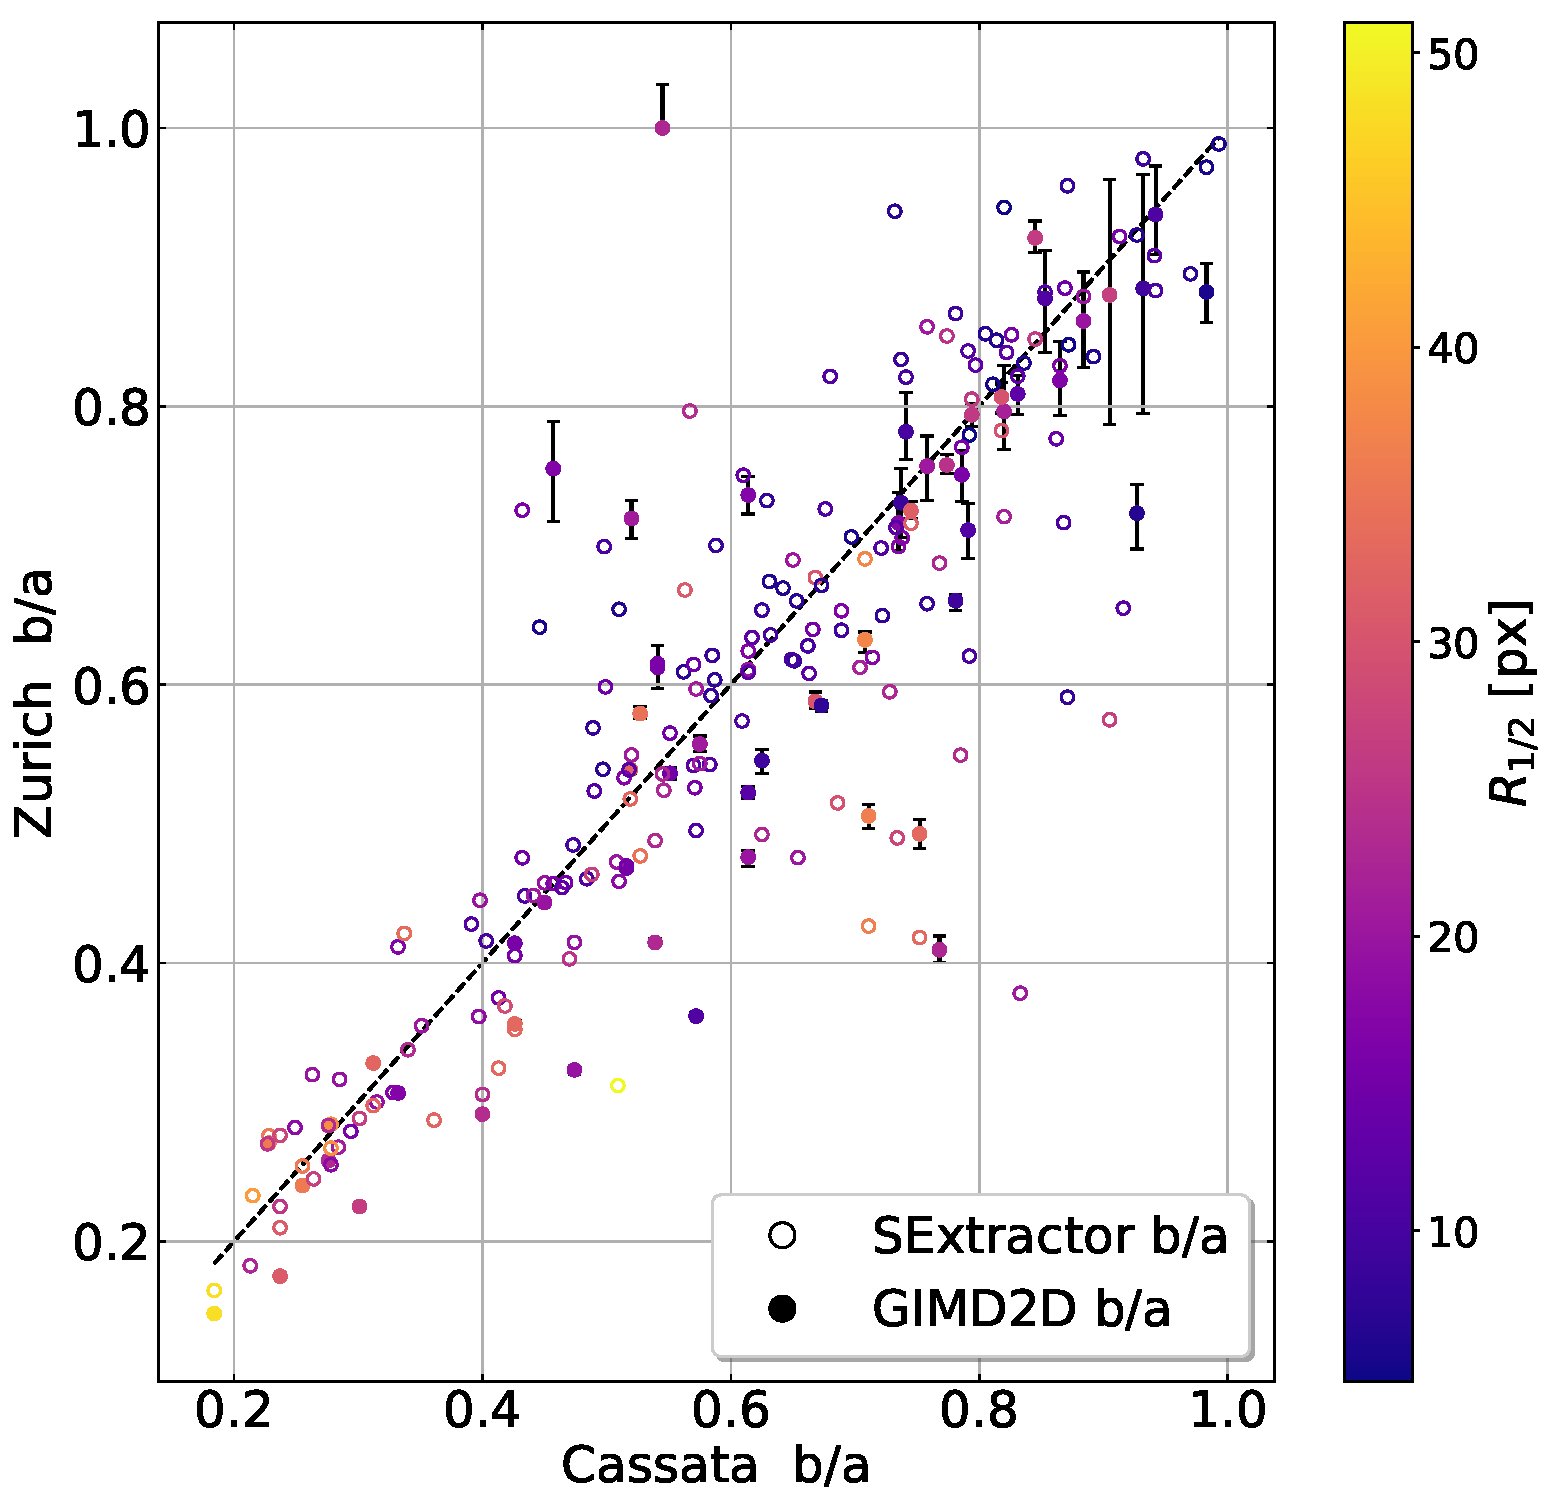
\includegraphics[width=\linewidth]{{graphics/check_b_a}.pdf}
			
			\begin{itemize}[label=$\rhd$]				
				\item values are consistent between catalogues
			\end{itemize}
		\end{column}
		
		\begin{column}{0.5\linewidth}
			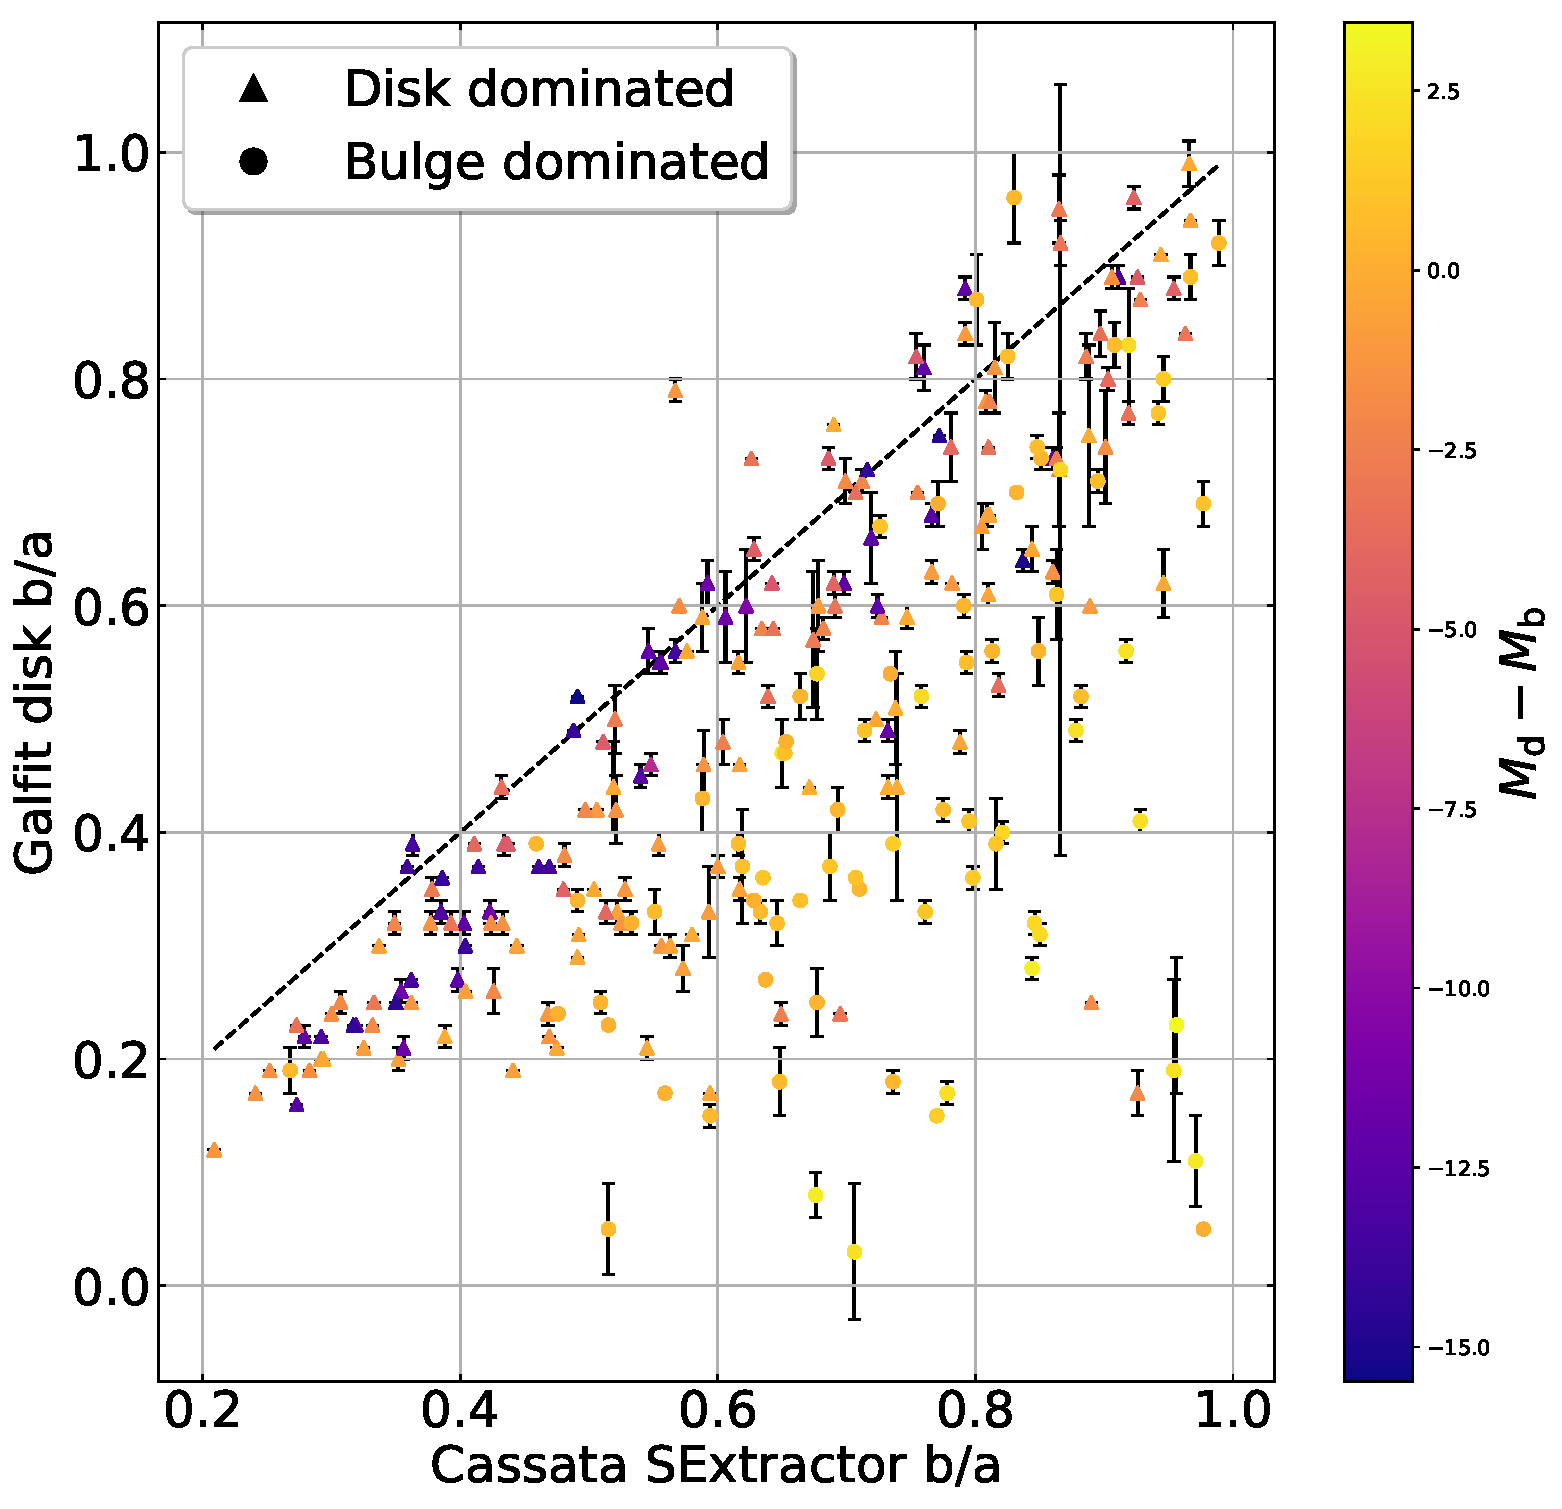
\includegraphics[width=\linewidth]{{graphics/check_b_a_GF}.pdf}
			
			\begin{itemize}[label=$\rhd$]				
				\item scatter is due to bulge dominated (spherically symmetric) systems
			\end{itemize}
		\end{column}
	\end{columns}
\end{frame}


\section{Characteristics of our sample}
\subsection{Redshift distribution}
\begin{frame}{Characteristics of our sample}
	\framesubtitle{Redshift distribution}
	\begin{columns}	
		\begin{column}{0.55\linewidth}
			\vspace{-10pt}		
			\begin{figure}
				\centering
				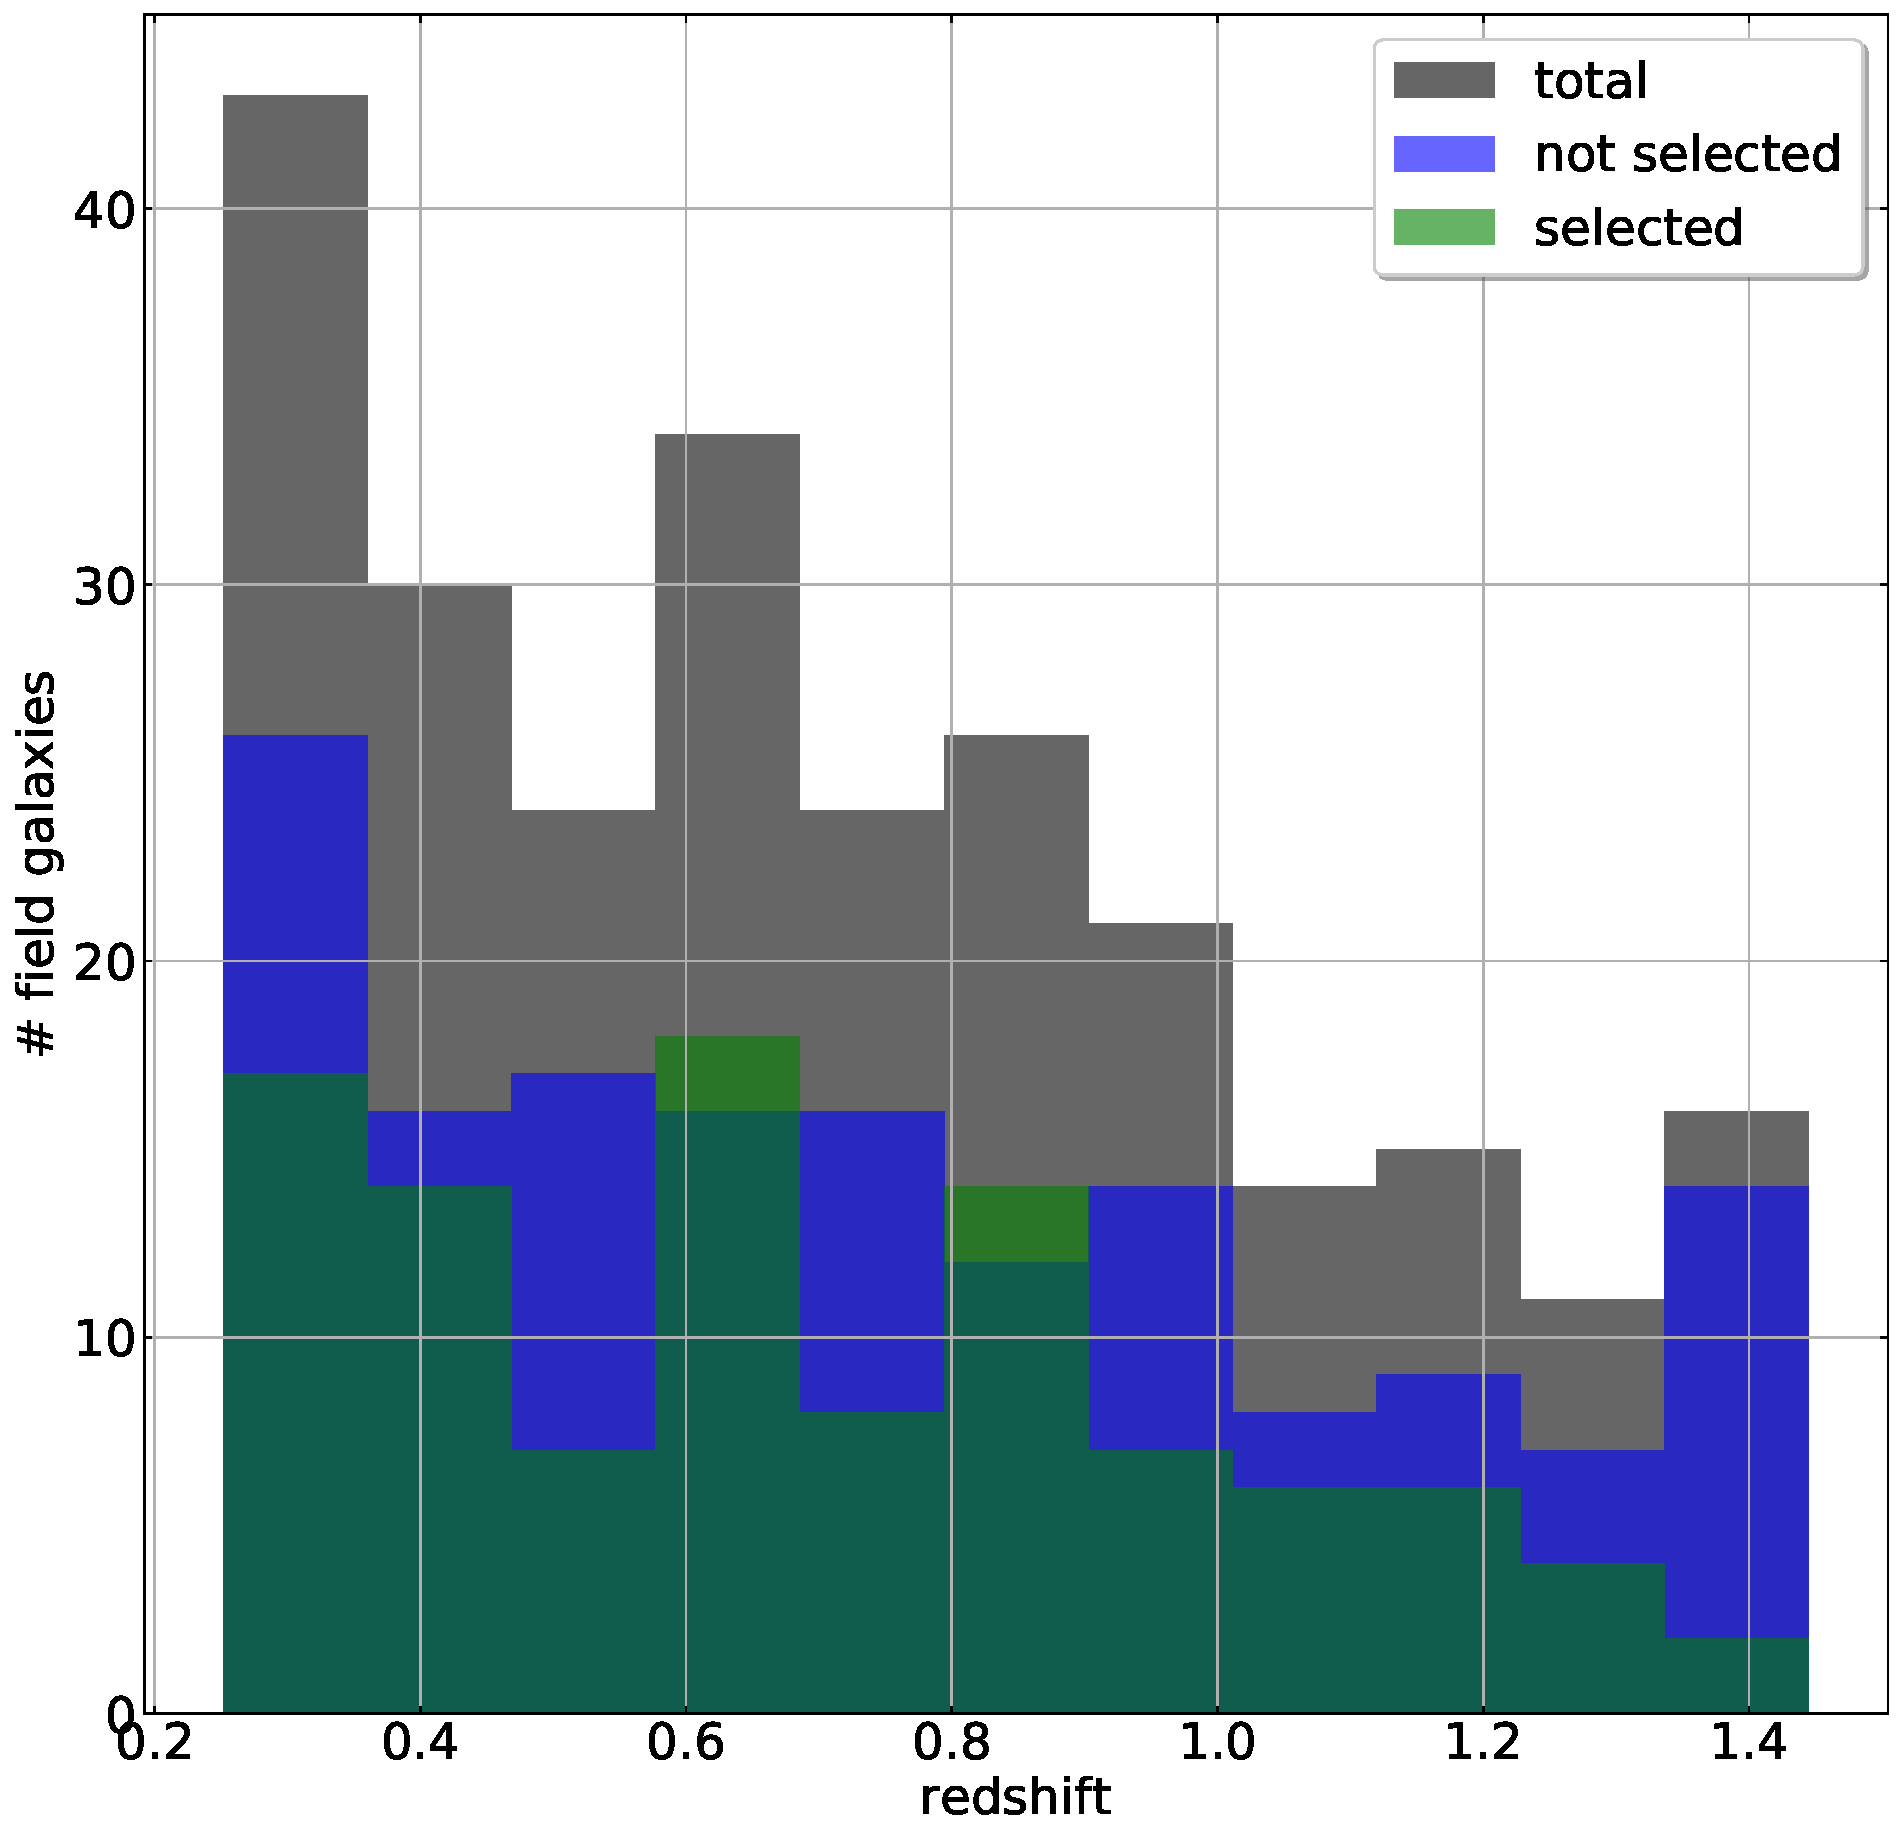
\includegraphics[width=\linewidth]{{graphics/hist_redshift}.pdf}
				\caption{The total number corresponds to galaxies with an HST counterpart in Cassata and/or Zurich catalogues.}
			\end{figure}
		\end{column}
		
		\begin{column}{0.5\linewidth}
			\begin{itemize}[label=$\rhd$]				
				\item sample of \textbf{103 galaxies} with $R_{\rm{1/2}} > \SI{0.35}{"}$ and $\rm{SNR} > 5$
				\item we loose galaxies at $z \approx 1.4$
				\item redshift distribution is not drastically changed
			\end{itemize}
		\end{column}
	\end{columns}

\end{frame}

\subsection{Mass-SFR relation}
\begin{frame}{Characteristics of our sample}
	\framesubtitle{Mass-SFR relation}
	\vspace{-3pt}
	\begin{columns}
		\begin{column}{0.4\linewidth}
			\begin{itemize}[label=$\rhd$]				
				\item Most of our sample galaxies are on the main sequence
				\item massive quiescent, low [OII] and very low mass galaxies are lost
			\end{itemize}
		\end{column}
		\begin{column}{0.6\linewidth}
		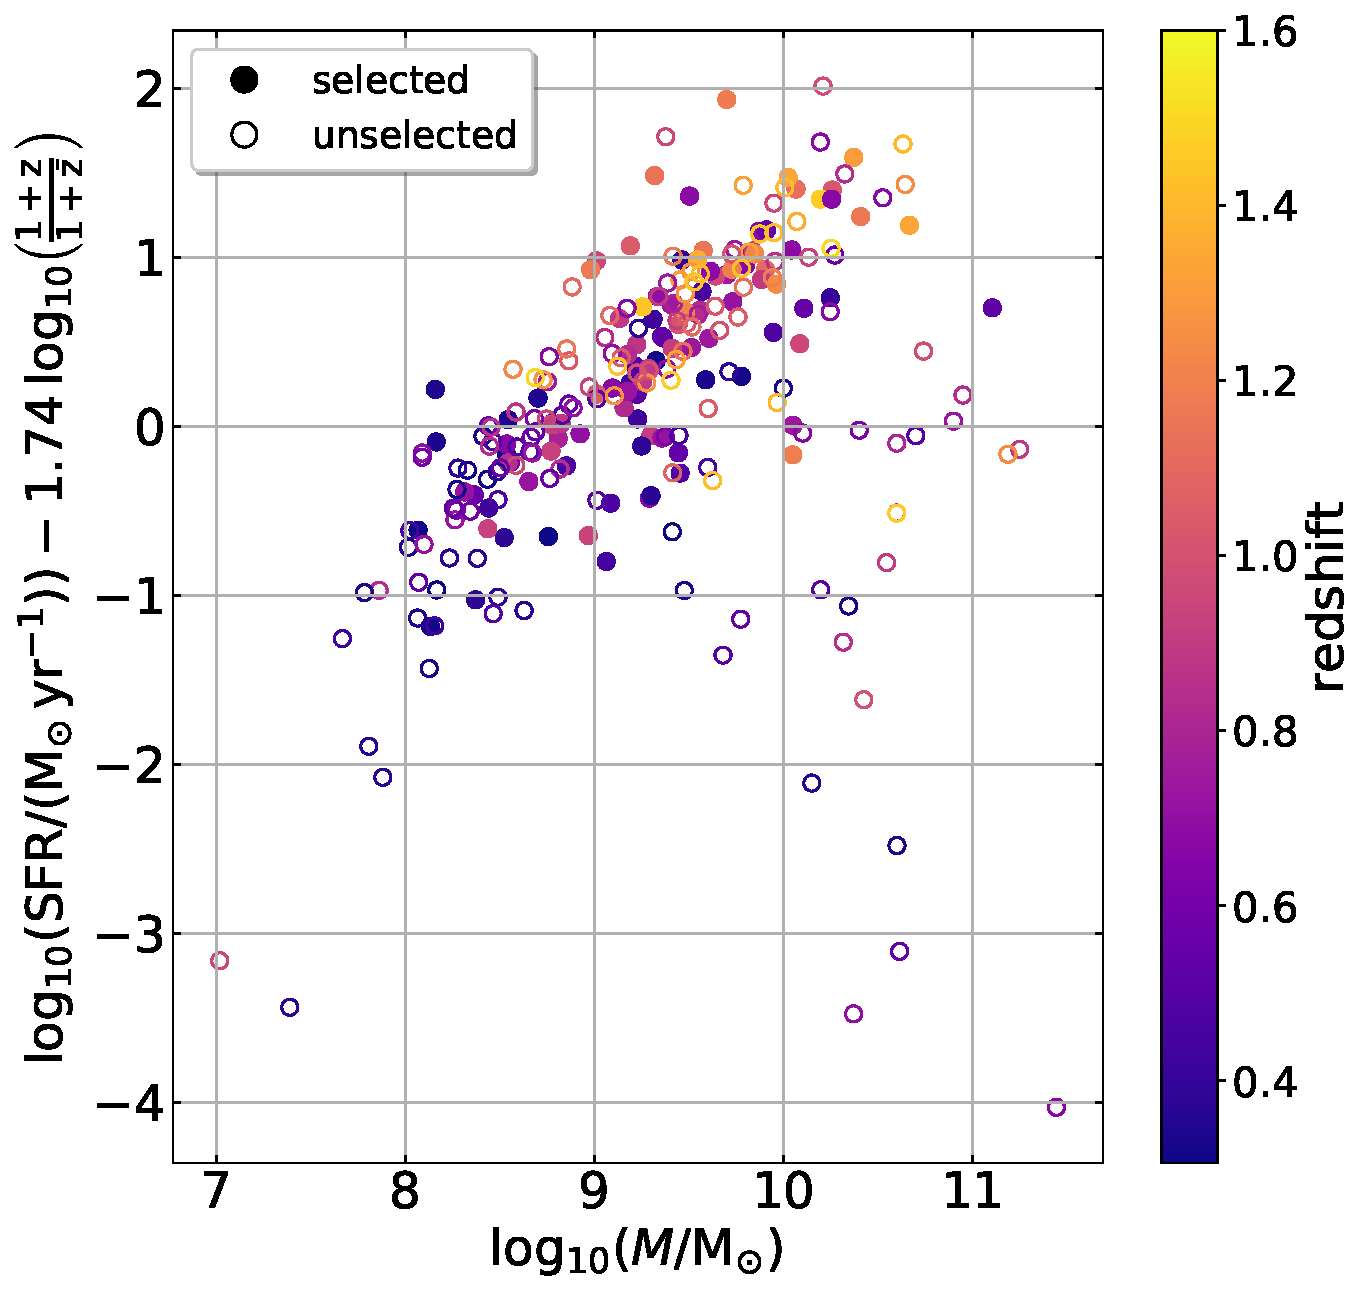
\includegraphics[width=\linewidth]{{graphics/SFR_vs_mass_correctedversiononly}.pdf}
		\end{column}

	\end{columns}
\end{frame}

\section{Kinematical modelling}
\subsection{Cleaning galaxies}
\begin{frame}{Kinematical modelling}
	\framesubtitle{Cleaning galaxies}
	\begin{columns}	
		\begin{column}{0.6\linewidth}
			\vspace{100pt}		
			\centering
			
\includegraphics[width=0.5\linewidth]{{graphics/VelBefore}.eps}
		\end{column}

		\begin{column}{0.6\linewidth}
			\vspace{100pt}		
			\centering
			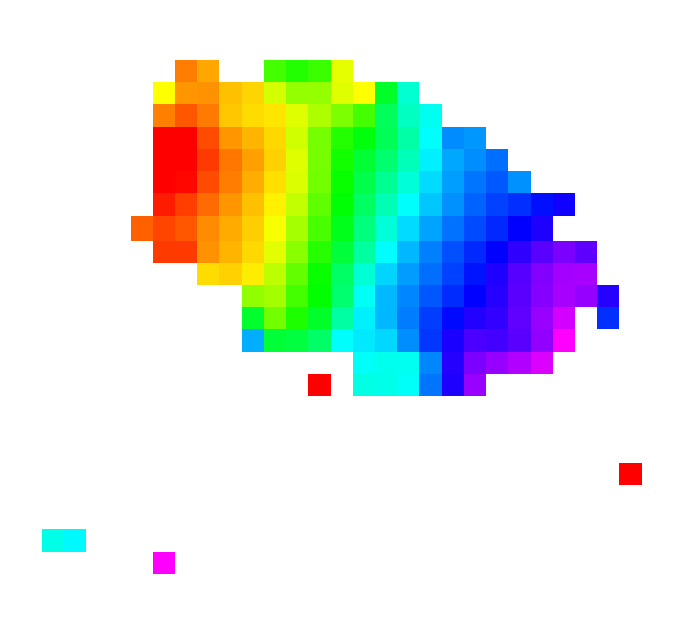
\includegraphics[width=0.5\linewidth]{{graphics/VelAuto}.eps}
		\end{column}
	\end{columns}
	
	\begin{textblock*}{5cm}(8.5cm,6cm)
		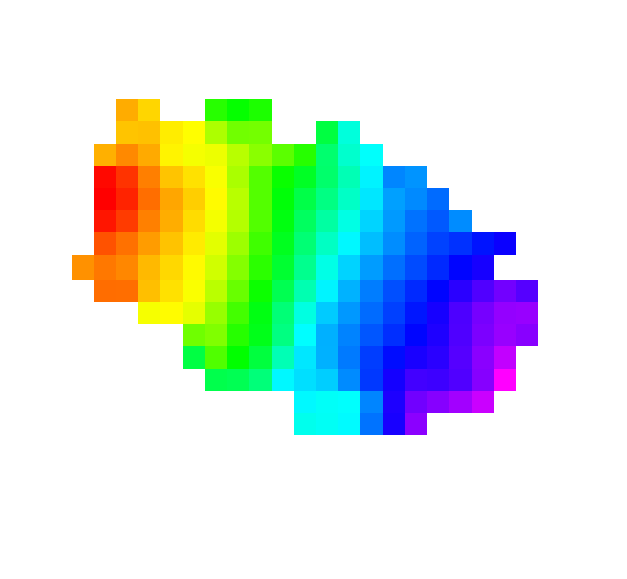
\includegraphics[width=0.6\linewidth]{{graphics/VelManual}.eps}
	\end{textblock*}
	
	%horizontal arrow and text
	\begin{textblock*}{5cm}(4.5cm,3cm)
		\centering
		\hspace{-10pt}
		Automatic \\
		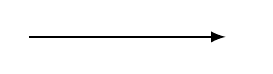
\begin{tikzpicture}[thick]
			\draw [black,   -latex      ] (0,7.0) -- (2.5,7.0) node [right] {};
		\end{tikzpicture}
	\end{textblock*}
	
	%vertical arrow
	\begin{textblock*}{5cm}(7.7cm,4.2cm)
		\centering
		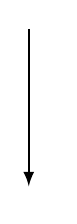
\begin{tikzpicture}[thick]
			\draw [black,   -latex      ] (0,9.0) -- (0.0,7.0) node [right] {};
		\end{tikzpicture}
	\end{textblock*}
	
	%vertical text
	\begin{textblock*}{5cm}(6.5cm,5.2cm)
		\centering
		Manual
	\end{textblock*}
	
	%three spectra
	\begin{textblock*}{7cm}(1cm,6.5cm)
		\centering
		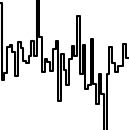
\includegraphics[width=0.25\linewidth]{{graphics/BadSpectrum}.png}
		\hfill
		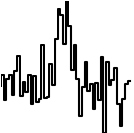
\includegraphics[width=0.25\linewidth]{{graphics/MediumSpectrum}.png}
		\hfill
		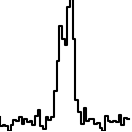
\includegraphics[width=0.25\linewidth]{{graphics/GoodSpectrum}.png}
	\end{textblock*}	
	
	%arrow for bad spectrum
	\begin{textblock*}{5cm}(-0.3cm, 4.3cm)
		\centering
		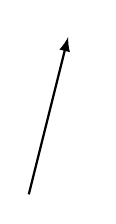
\begin{tikzpicture}[thick]
			\draw [black,   -latex      ] (0,7.0) -- (0.5,9) node [right] {};
		\end{tikzpicture}
	\end{textblock*}
	
	%arrow for medium spectrum
	\begin{textblock*}{5cm}(1cm, 3.9cm)
		\centering
		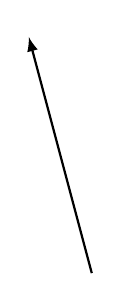
\begin{tikzpicture}[thick]
			\draw [black,   -latex      ] (0.8,7.0) -- (0,10) node [right] {};
		\end{tikzpicture}
	\end{textblock*}
	
	%arrow for medium spectrum
	\begin{textblock*}{5cm}(2.5cm, 3.3cm)
		\centering
		\begin{tikzpicture}[thick]
			\draw [black,   -latex      ] (4.5,7.0) -- (1,10.5) node [right] {};
		\end{tikzpicture}
	\end{textblock*}
	
	
\end{frame}

\subsection{Fitting a model}
\begin{frame}{Kinematical modelling}
	\framesubtitle{Fitting a model}
	\centering
	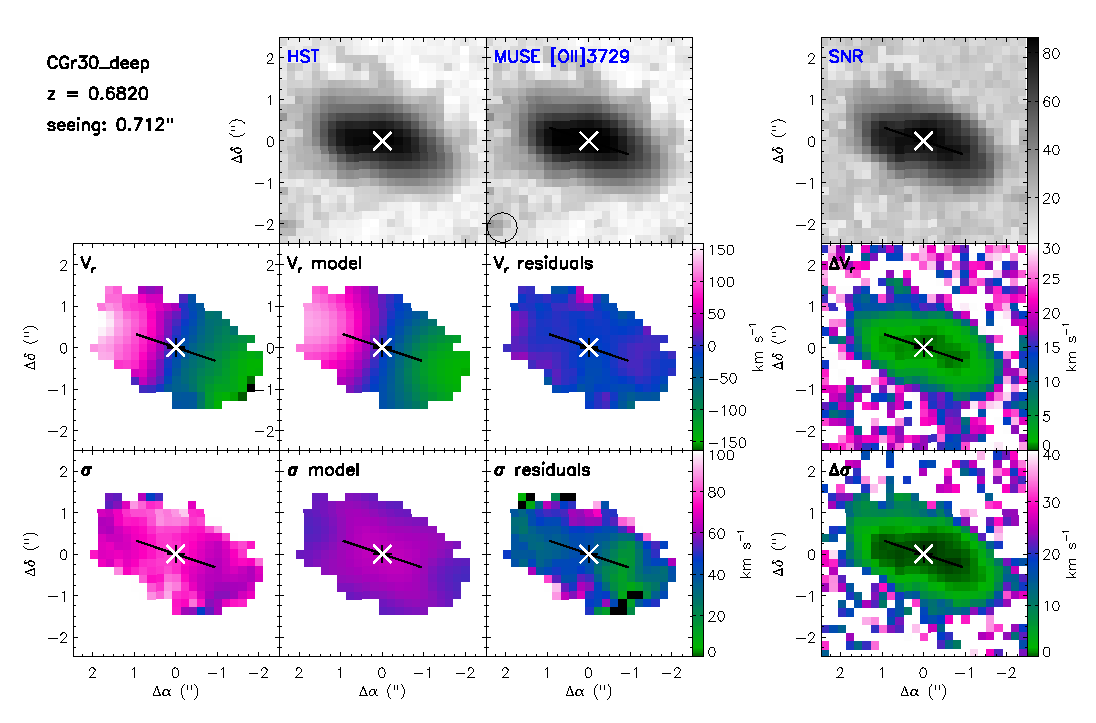
\includegraphics[width=0.8\linewidth]{{graphics/maps_CGr30_deep_91_o2_paper}.eps}

\end{frame}

\section{First results}
\subsection{$V_{\rm{max}}/\sigma_{\rm{v}}$ distribution}
\begin{frame}{First results}
	\framesubtitle{$V_{\rm{max}}/\sigma_{\rm{v}}$ distribution}

\end{frame}

\subsection{Tully-Fisher relation}
\begin{frame}{First results}
	\framesubtitle{Tully-Fisher relation}
\end{frame}

\begin{frame}[t,allowframebreaks]
\frametitle{Bibliography}

\nocite{*} % will display the non-cited publications as well. Useful for a publication list.

\printbibliography

\end{frame}
\end{document}